\documentclass{beamer}

\usetheme{Pk}

\newcommand\rb[1]{\textcolor{ThemeRed}{\textbf{#1}}}
\newcommand\gr[1]{\textcolor{ThemeGrey}{#1}}
\usepackage{listings}
\lstset{
  basicstyle=\scriptsize,
  columns=fullflexible,
  showstringspaces=false,
  commentstyle=\color{ThemeGrey}\upshape
}

\lstdefinelanguage{XML}
{
  morestring=[b]",
  moredelim=[s][\color{ThemeGreen}]{<}{\ },
  moredelim=[s][\color{ThemeGreen}]{</}{>},
  moredelim=[l][\color{ThemeGreen}]{/>},
  moredelim=[l][\color{ThemeGreen}]{>},
  stringstyle=\color{ThemeBlue},
  identifierstyle=\color{ThemeGreen},
  keywordstyle=\color{ThemeRed},
}

\hypersetup{
  colorlinks = true,
  linkcolor = ThemeGrey,
  urlcolor = ThemeLightBlue
}   


\title{Open Data Management \& Cloud\\exam project}
\subtitle{Audio music file archiving}
\author{Patrick Indri}
\date{\today}


\begin{document}
	\setcounter{showSlideNumbers}{0}

	\frame{\titlepage}

	\setcounter{framenumber}{0}
	\setcounter{showSlideNumbers}{1}



\section{Introduction}

  \begin{frame}
    \frametitle{Contents}
    
    The presentation is organised as follows:
    
    \vspace{1em}
    
    \begin{enumerate}
      \item Introduction
      \begin{itemize}
        \item[] \gr{Aim and project description}
      \end{itemize}
      \item Model design and implementation
      \begin{itemize}
        \item[] \gr{UML, XSD and XML}
      \end{itemize}
      \item Interfaces and services
      \begin{itemize}
        \item[] \gr{Search filter, data annotation and storage}
      \end{itemize}
      \item Preservation and interoperability
      \begin{itemize}
        \item[] \gr{Metadata preservation, semantic interoperability and audio file formats}
      \end{itemize}
      \item Final considerations
    \end{enumerate}


  \end{frame}



  \begin{frame}
    \frametitle{Introduction}

    \begin{block}{Aim of the project}
      Investigation of audio file archiving for music.
    \end{block}

    \vspace{1em}

    In particular:
    \begin{itemize}
      \item UML metadata model;
      \item XSD implementation and XML sample document;
      \item discussion of data discovery/access and interoperability;
      \item discussion of (long term) archiving and data preservation.
    \end{itemize}

    \vspace{1em}

    \rb{Data resource:} not an actual dataset but music files in general.

  \end{frame}



  \begin{frame}
    \frametitle{Metadata standards for audio files}

    There is no widely used and standardised metadata model for music audio files.

    \vspace{1em}

    \begin{itemize}
      \itemsep1em
      \item Dublin Core: simple (15 terms), focus on descriptive metadata;
      \item EbuCore: detailed DC extension, fine grain technical and administrative metadata for broadcasting;
      \item METS: handles the structural/hierarchical metadata of a digital library. Open flexibility (no vocabulary).
    \end{itemize}
  \end{frame}



\section{Model design and implementation}


  \begin{frame}
    \frametitle{Model design}

    What should the data model represent?

    \vspace{1em}

    \begin{itemize}
      \itemsep0.75em
      \item Songs and their different versions;
      \item Groups of songs (releases);
      \item Artists;
      \item Basic technical metadata;
      \item Relations between songs, releases and artists.
    \end{itemize}

  \end{frame}



  \begin{frame}
    \frametitle{UML}
    \begin{center}
      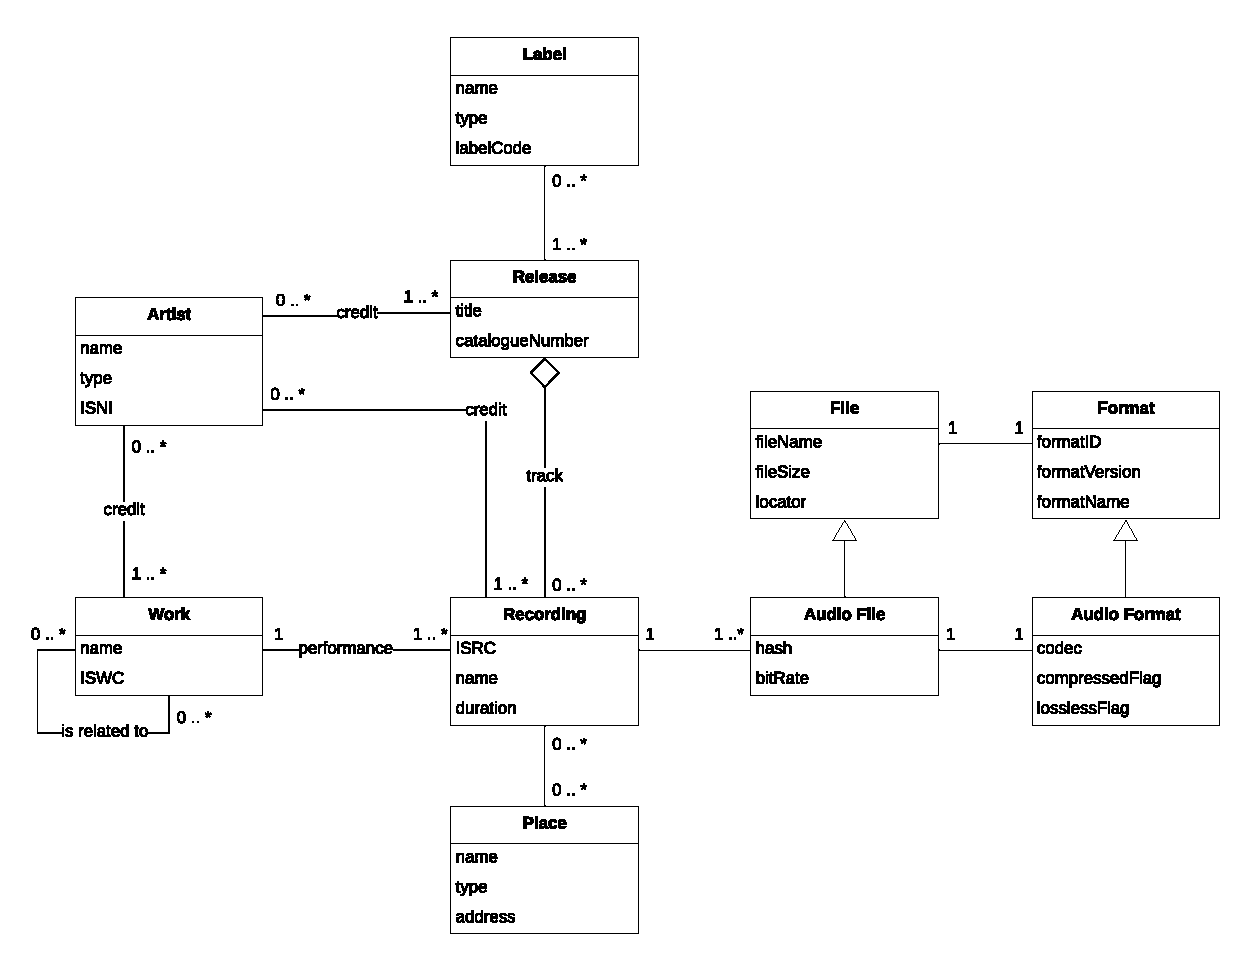
\includegraphics[width=0.95\textwidth]{img/UML.pdf}
    \end{center}
  \end{frame}



  \begin{frame}
    \frametitle{XSD}

    Choice of implementation:

    \vspace{0.5em}

    \begin{itemize}
      \item RDB: easy to enforce constraints (primary/foreign keys), widely used, easy to model relationships, rigid structure;
      \item \rb{XSD}: flexible, easily handle partial data, harder relationship handling.
    \end{itemize}

    \vspace{1.5em}

    The proposed XSD implementation should:

    \vspace{0.5em}

    \begin{itemize}
      \item Refine Dublin Core;
      \item Balance integrity constraints and partial data;
      \item Model relationships with detail. 
    \end{itemize}

    \vspace{1.5em}

    The resulting XSD can be retrieved \href{https://github.com/pindri/ODMC_exam/blob/master/odmc.xsd}{here}.
  \end{frame}




  \begin{frame}[fragile]
    \frametitle{XML example}

    Example of an XML document, valid against the proposed XSD.

    \vspace{0.5em}

    \lstset{basicstyle=\small}
\begin{lstlisting}[language=XML]
<work>
  <ISWC id="ISWC_T-000.000.000-A"></ISWC>
  <title lang="en">
    <dc:title>Test Work</dc:title>
  </title>
  <hasArtist label="Will Wilson" description="Singer">
  </hasArtist>
  <hasPerformance label="Test Rec." description="Studio Ver.">
    <relationIdentifier>
      <ISRC idref="ISRC_AAAAA0000000"></ISRC>
    </relationIdentifier>
  </hasPerformance>
</work>
\end{lstlisting}

    \vspace{1em}

    The KEY/KEYREF approach was used to model the relationships.
  \end{frame}



  \begin{frame}
    \frametitle{Difficulties and possible expansions}
    
    \textcolor{red}{Difficulties:}
    
    \vspace{0.5em}
    
    \begin{itemize}
      \item flexibility;
      
    \end{itemize}

    \vspace{1em}
    
    Possible expansions:
    
    \vspace{0.5em}
    
    \begin{itemize}
      \item Include sort names;
      \item Include pictures for artists and releases;
      \item KEY/KEYREF cross domain.
    \end{itemize}

  \end{frame}



\section{Interfaces and Services}

  \begin{frame}
    \frametitle{Data discovery: search/filter service}

    The most fundamental service would be a search/filter service.

    \vspace{0.5em}

    \begin{itemize}
      \item Free text queries on the various categories (artist, release, work, recording);
      \item Queries can be implemented using XQuery;
      \item Information retrieval techniques to improve results: edit distance and k-gram distance for spelling correction;
      \item Popularity rank for the results.
    \end{itemize}


    \vspace{1em}

    Once the resource has been identified: download (lossy and lossless file) and online preview.

    \vspace{1em}

    \rb{Crucial point:} XML indexing, trade-off between memory usage and performance.

  \end{frame}



  \begin{frame}
    \frametitle{Data annotation}

    Metadata can be embed in audio files. \rb{Is it advisable?} A minimal amount, the \textit{catastrophic} metadata is necessary. Most metadata should be saved in external files.

    \vspace{1em}

    Viable metadata containers:

    \vspace{0.5em}

    \begin{itemize}
      \item ID3: designed for Mp3, highly structured;
      \item XMP: ISO standard for JPEG images, defined for other formats including Mp3 and WAW;
      \item BWF \texttt{<bext>} chunk: XML administrative metadata for BWF;
      \item Vorbis comments: unstructured metadata for Vorbis and FLAC.
    \end{itemize}

    \vspace{1em}

    \rb{Conclusion:} data annotation heavily depends on file format choice.

  \end{frame}



  \begin{frame}
    \frametitle{Storage and Cloud Solutions}

    Storing \rb{XML} files:

    \vspace{0.5em}

    \begin{itemize}
      \item XML-native databases are not scalable;
      \item XML-enabled databases are well established, scalable and can be queried with SQL;
    \end{itemize}

    \vspace{0.5em}

    \rb{Crucial point:} the proposed XSD itself is not scalable.

    \vspace{1em}

    \rb{Audio} files can be stored in BLOBs in the database: not flexible. Alternatively:

    \vspace{0.5em}

    \begin{itemize}
      \item Up to \textit{few} TB: remote filesystem;
      \item Large archives: distributed DB;
      \item Cloud solutions: Amazon S3 offers versioning, orphan files handling, redundancy and access control.
    \end{itemize}

  \end{frame}



\section{Preservation and Interoperability}

  \begin{frame}
    \frametitle{Data preservation}

    A primary concern for an audio archive. The proposed XSD prevent data duplication and limits orphan data.

    \vspace{1em}

    Most technical and descriptive metadata is \rb{stable} and, in principle, it is not essential to preserve it. Catastrophic metadata is \rb{ephemeral} (e.g., the ISRC for a recording) and must be preserved.

    \vspace{1em}

    Audio file hashes can be used to check file integrity.

    \vspace{1em}

    Cloud solutions for \rb{long term preservation}: AWS S3 Glacier and Glacier Deep.
    
    \vspace{1em}

    \rb{Crucial point:} an OAIS implementation could not be \textit{open access} for copyrighted files.

  \end{frame}


  
  \begin{frame}
    \frametitle{Interoperability}

    The proposed model strives for semantic interoperability.

    \vspace{1em}

    \begin{itemize}
      \itemsep0.5em
      \item Syntactic interoperability: XML is an open format;
      \item Semantic interoperability: XSD equips data with meaning, Dublin Core support;
      \item Standardised and persistent identifiers for the principal classes;
    \end{itemize}

    \vspace{1em}

    A report is associated with the project: it provides ontological information on the model.
  \end{frame}

  

  \begin{frame}
    \frametitle{Audio file formats}
    
    One of the most crucial design choices: obsolete and proprietary file formats make data handling troublesome (\textit{digital dark age}).

    \vspace{1em}

    (Quasi) open file formats should be used:

    \vspace{0.5em}

    \begin{itemize}
      \itemsep0.5em
      \item BFW: uncompressed extension of Microsoft WAW, open format;
      \item FLAC: smaller file size, compressed lossless format, good metadata support;
      \item MP3: most popular audio file format, very small file size, lossy compression, non a viable alternative for archiving (good for download/preview).
    \end{itemize}

    \vspace{1em}

    \rb{Crucial point:} the file format should be well established;

  \end{frame}

  

\section{Final considerations}

  \begin{frame}
    \frametitle{Final considerations}
    
    Audio file data management is difficult because:
    
    \vspace{1em}
    
    \begin{itemize}
      \itemsep1em
      \item Many impact design choices;
      \item Lack of metadata standard can make interoperability difficult;
      \item Practical issues: storage and indexing;
      \item Cloud solutions to deal with large volumes and concurrent access.
    \end{itemize}

  \end{frame}



\end{document}
